\section{Experiment Steps}
\label{sec:steps}
%-------------------------------------------------------------------------
In this experiment, we mainly use Faster R-CNN and YOLO for testing. First, we match the existing models with the experimental tasks, complete the baseline reproduction, and then adjust and innovate the models. Through ablation experiments, we compare and find the best results.

\subsection{Environment Configuration}
\noindent
\textbf{Python:} 3.11.8

\noindent
\textbf{GPU:} RTX4090

\subsection{Model Configuration}
\subsubsection{Faster R-CNN}
\noindent
\textbf{Model:} Faster R-CNN with ResNet-50-FPN backbone

\noindent
\textbf{Dataset:}

\noindent
Training image path:

/home/zgm2024/CVpj/train/images

\noindent
Label file path:

/home/zgm2024/CVpj/train/label\_train.json

\noindent
\textbf{Data Processing:} Custom dataset class TamperingDataset is used to load images and annotations, and skip images with regions smaller than 10 pixels.

\noindent
\textbf{Training Settings:}

\noindent
Loss function:

Sum of classification and regression losses of Faster R-CNN

\noindent
Optimizer:

AdamW, initial learning rate $lr = 0.001$, weight decay $weight\_decay = 0.01$

\noindent
Scheduler:

StepLR, decay factor of 0.1 every 3 epochs, i.e., $step\_size = 3,\ gamma = 0.1$

\noindent
Batch size: 4

\noindent
Device: GPU (if available)

\noindent
\textbf{Pre-trained Weights:} The model is initialized from torchvision's pre-trained weights

\noindent
\textbf{Output:}

\noindent
The trained model is saved at the path:

/home/zgm2024/CVpj/train/model/tampering\_detection\_
model\_updated.pth

\subsubsection{YOLO}
\noindent
\textbf{Model:} YOLOv8n

\noindent
\textbf{Dataset Configuration:}

\noindent
YAML configuration file path:

/home/zgm2024/CVpj/yolo/datasets/yolo\_config.yaml

\noindent
\textbf{Training Settings:}

\noindent
Initial uniform image size: 640$\times$640 pixels

\noindent
Batch size: 16

\noindent
Device: GPU 0

\noindent
\textbf{Pre-trained Weights:} Initialized from yolov8n.pt

\noindent
\textbf{Output:}

\noindent
Training logs and weights are saved at:

/home/zgm2024/CVpj/yolo/runs/train/tampering\_detection

\subsection{Baseline Reproduction}

In this section, we perform baseline reproduction for the Faster R-CNN and YOLO models, changing only the number of training epochs to observe the training effects and select the better model.

\subsubsection{Faster R-CNN}

The model is trained with parameters $lr = 0.001,\ weight\_decay = 0.01,\ step\_size = 3,\ gamma = 0.1$. The training epochs are gradually increased, and the relationship between Micro-F1 score and the number of epochs for the Faster R-CNN model is shown in the line chart \cref{fig:faster-r-cnn}.
\begin{figure}[t]
  \centering
  %\fbox{\rule{0pt}{2in}
  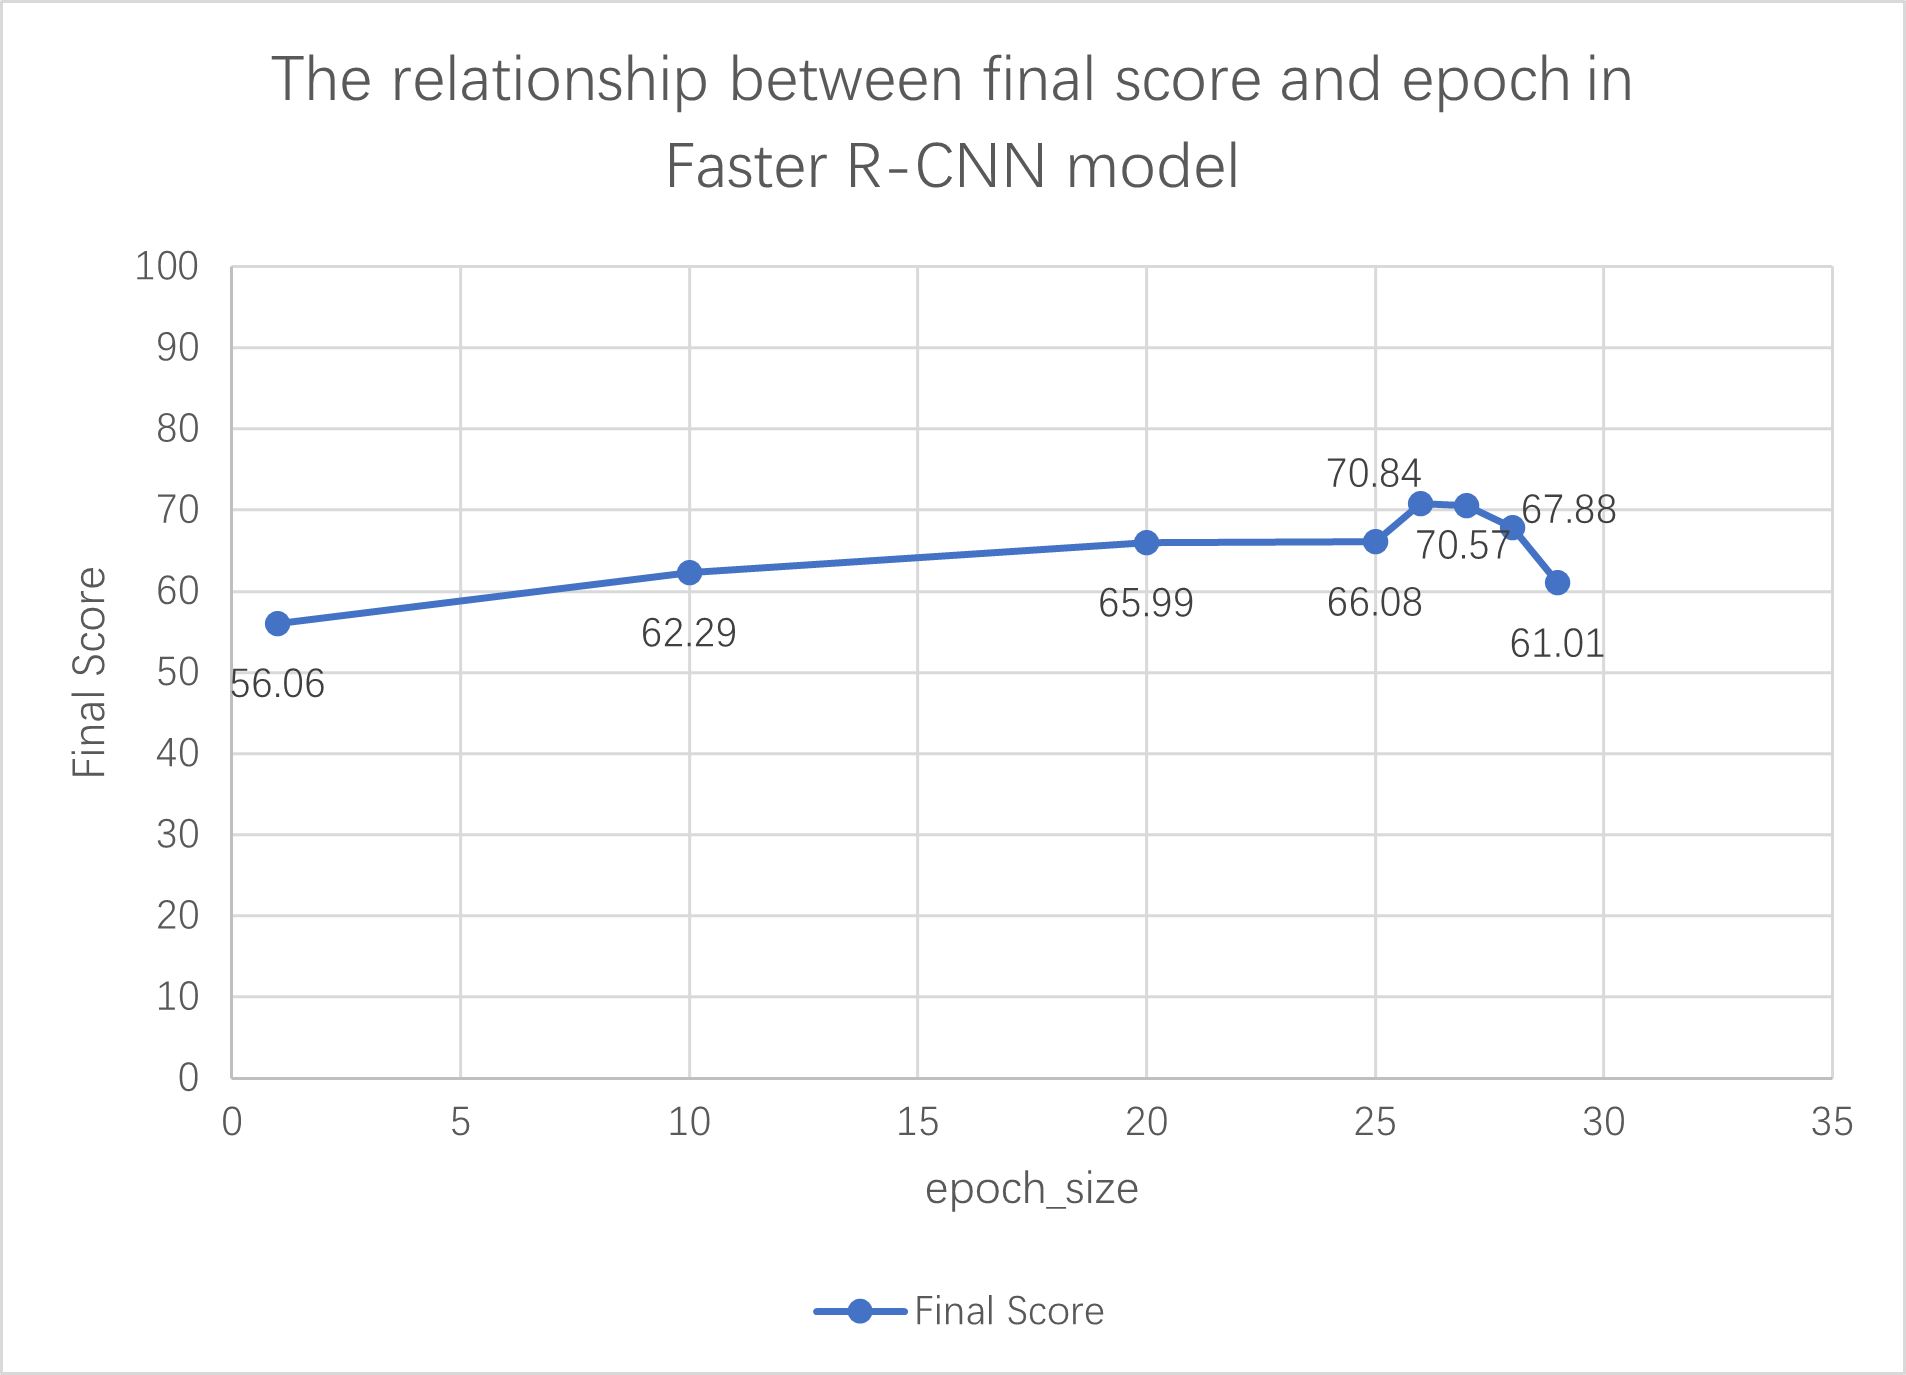
\includegraphics[width=0.8\linewidth]{./graphs/图片1.png}
  %\rule{0.9\linewidth}{0pt}
  %}

  \caption{Micro-F1 vs. Epochs for Faster-RCNN Model}
  \label{fig:faster-r-cnn}
\end{figure}

The initial Micro-F1 score of the Faster R-CNN model is 56.06. By increasing the epochs, we find that at epoch 26, the score reaches the maximum of 70.84. After further training, the score decreases, indicating that the model may have overfitted.

The Faster R-CNN model is easy to call and has a simple model definition. After 26 epochs, the model achieves the best score, but the training process is slow. Data augmentation significantly increases training time, and the results are not ideal. However, Faster R-CNN helps to understand the ResNet-50 network structure and the significance of hyperparameter tuning for model training.

\subsubsection{YOLOv8n}

Training with parameters $imgsz = 640,\ batch = 16$ and predicting with parameter $conf = 0.25$, we gradually increase the training epochs. The relationship between Micro-F1 score and epochs for the YOLOv8n model is shown in the line chart \cref{fig:yolov8n}.
\begin{figure}[t]
  \centering
  %\fbox{\rule{0pt}{2in}
  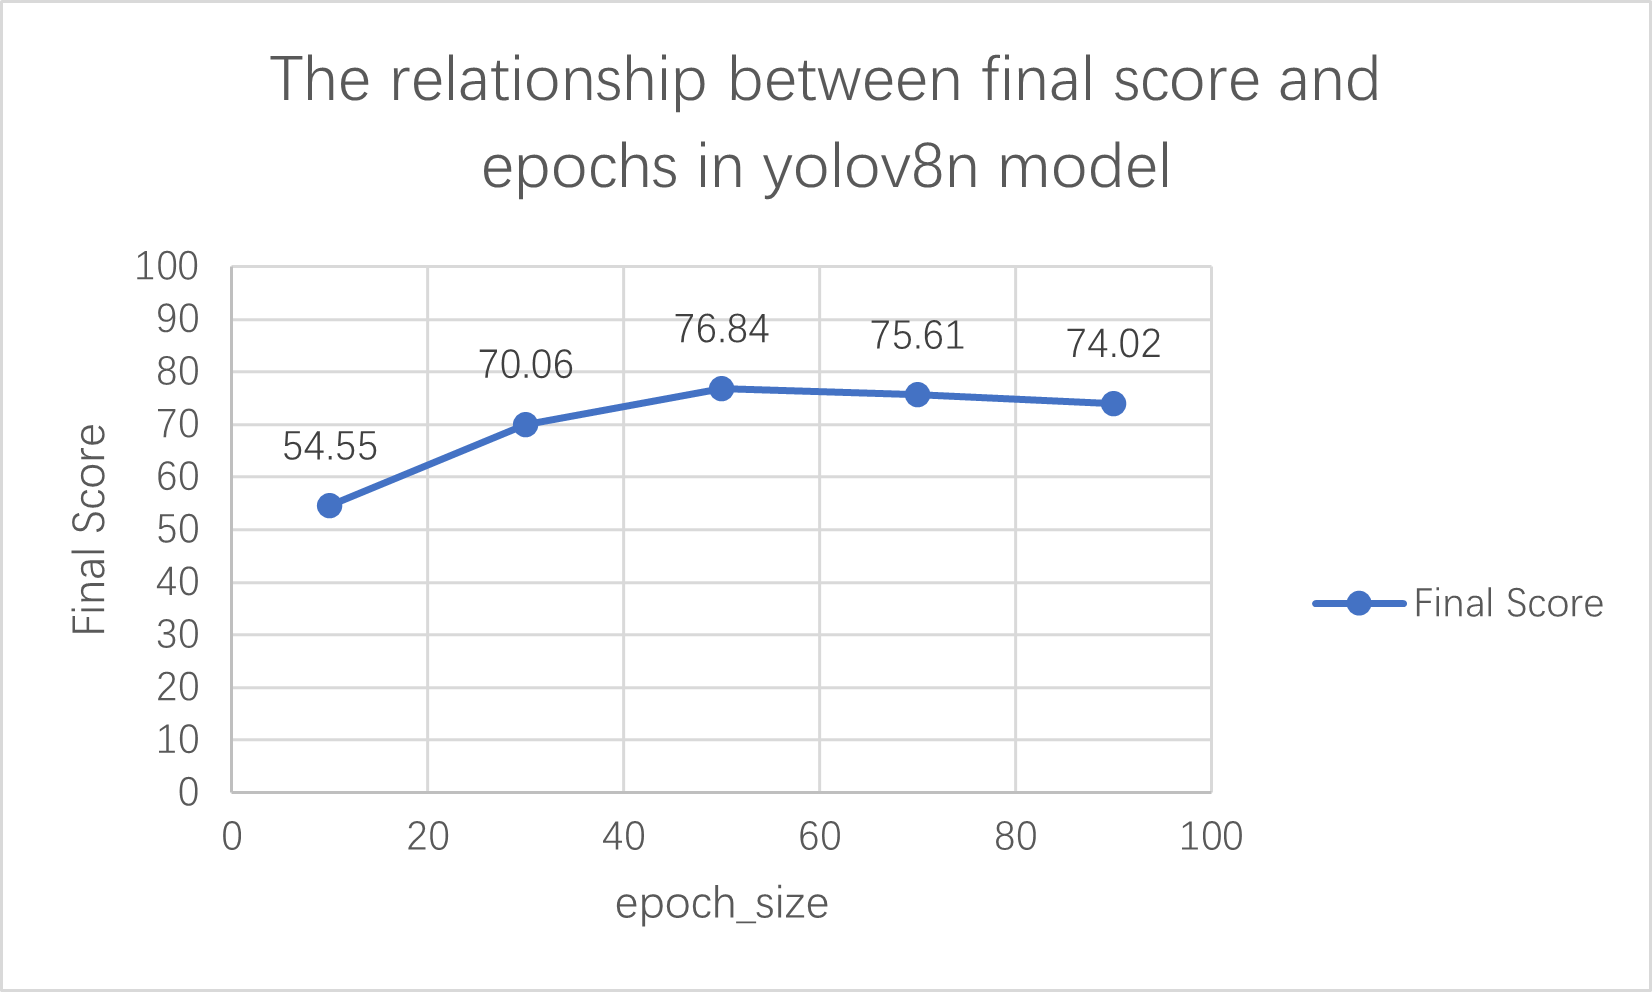
\includegraphics[width=0.8\linewidth]{./graphs/图片2.png}
  %\rule{0.9\linewidth}{0pt}
  %}

  \caption{Micro-F1 vs. Epochs for YOLOv8n Model}
  \label{fig:yolov8n}
\end{figure}

The number of training epochs has a significant effect on the score. After rough estimation, the model reaches its maximum score of 76.84 after around 50 epochs, surpassing Faster R-CNN. The YOLOv8n model trains much faster than Faster R-CNN, proving that the YOLO model is more flexible. Therefore, we consider using a larger model for training based on YOLO.

\subsubsection{YOLO Model Version Comparison}

Based on the YOLO model, we attempt to train with larger and newer models. Based on the baseline experiment results of YOLOv8n, we train YOLO11n and YOLO11m, and compare the results of epoch 50 and epoch 70 in a bar chart \cref{fig:yolo-compare}.
\begin{figure}[t]
  \centering
  %\fbox{\rule{0pt}{2in}
  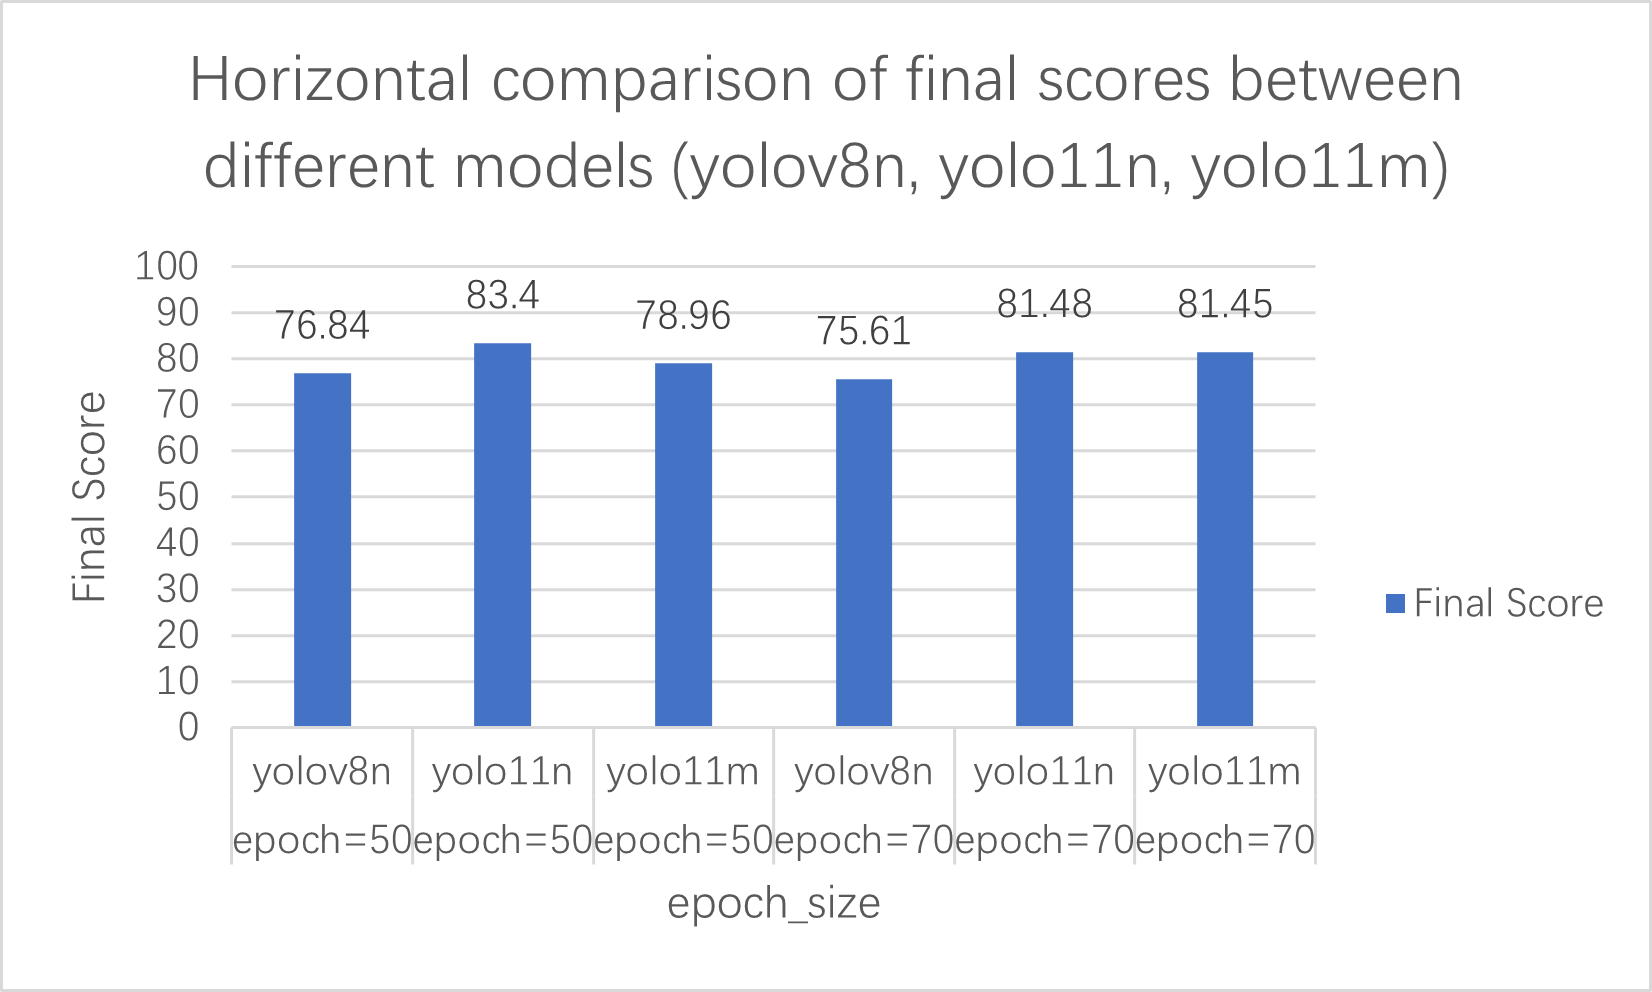
\includegraphics[width=0.8\linewidth]{./graphs/图片3.png}
  %\rule{0.9\linewidth}{0pt}
  %}

  \caption{Comparison of YOLOv8n, YOLO11n, and YOLO11m}
  \label{fig:yolo-compare}
\end{figure}

From the chart, it is clear that for the updated YOLO11 model, the accuracy is significantly higher than YOLOv8 when all other parameters are consistent. Although YOLO11m has a larger number of parameters, its accuracy is lower than YOLO11n in the chart. This suggests that the accuracy of the model is not only related to the number of parameters but also to other parameters (such as epoch and batch). When the epoch and batch are smaller, YOLO11m does not necessarily outperform YOLO11n. The subsequent \cref{subsec:create} section will carefully compare the effects of epoch and batch on YOLO11m, as the highest score is achieved by YOLO11m.

\subsection{Method Innovation}
\label{subsec:create}
\subsubsection{Innovation 1: Region Threshold Filtering}
To improve the model's detection performance on different images and provide multiple detection intervals, we modify the Faster R-CNN evaluation logic to set a confidence threshold for generating tampered regions. The code modification is shown in \cref{fig:faster-r-cnn-conf-code}.
\begin{figure}[t]
  \centering
  %\fbox{\rule{0pt}{2in}
  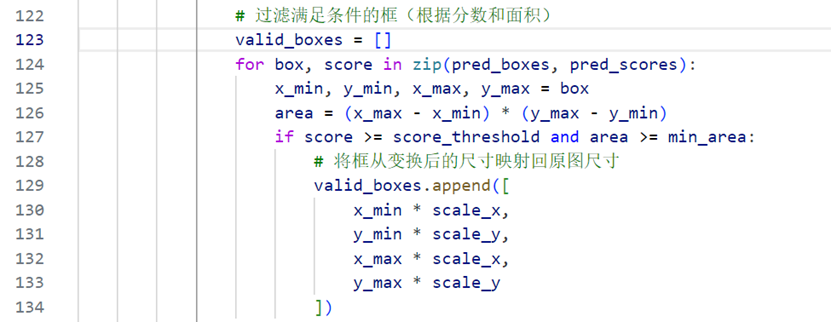
\includegraphics[width=0.8\linewidth]{./graphs/图片4.png}
  %\rule{0.9\linewidth}{0pt}
  %}

  \caption{Code Modification for Region Threshold Filtering}
  \label{fig:faster-r-cnn-conf-code}
\end{figure}

From the highest score point in \cref{fig:faster-r-cnn}, we compare the 26th and 27th epochs with and without region threshold filtering. The results are shown in the bar chart \cref{fig:faster-r-cnn-conf}.
\begin{figure}[t]
  \centering
  %\fbox{\rule{0pt}{2in}
  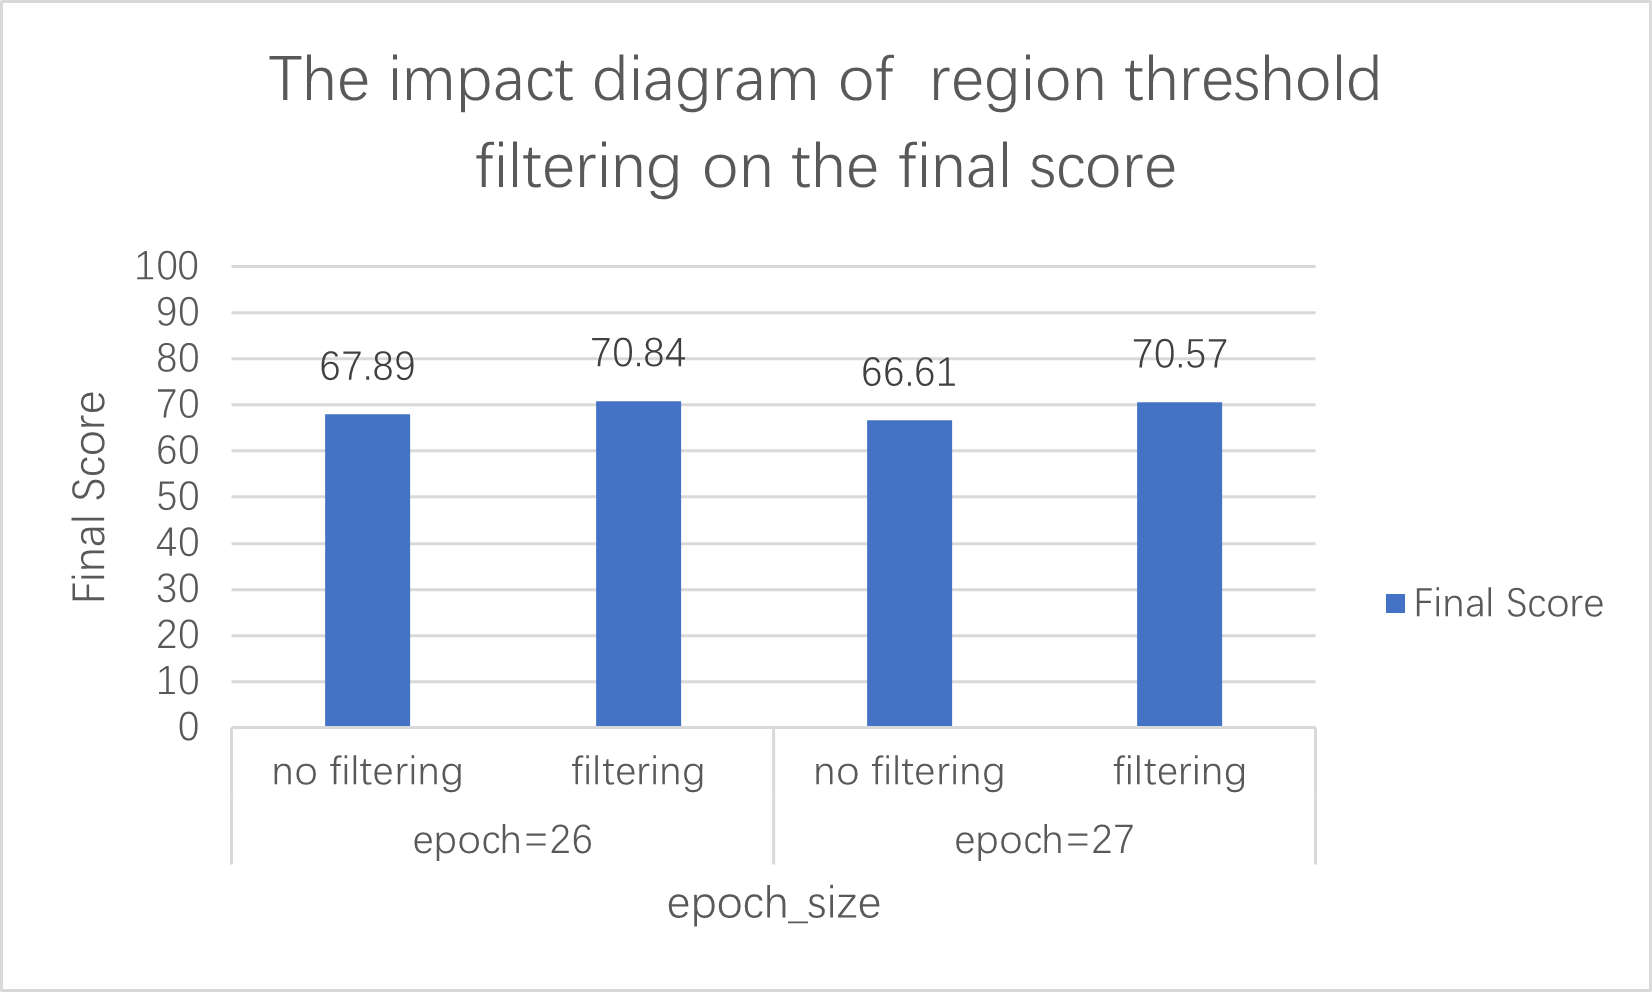
\includegraphics[width=0.8\linewidth]{./graphs/图片5.png}
  %\rule{0.9\linewidth}{0pt}
  %}

  \caption{Impact of Region Threshold Filtering in Faster R-CNN}
  \label{fig:faster-r-cnn-conf}
\end{figure}

From the chart, we can see that the score has significantly improved with the innovation of region threshold filtering, indicating that this method has a clear effect in this experiment.

\subsubsection{Innovation 2: Adjusting Training Parameters and Configuration Files}
In this section, we adjust the parameters for YOLO11m and gradually converge to the highest possible score for the YOLO model.

First, we modify the batch size and increase the number of training epochs. These two parameters have a significant impact on the prediction score. We train with batch sizes of 64 and 256 for 40, 60, and 80 epochs, and the results are shown in the bar chart \cref{fig:yolo-batchsize}.
\begin{figure}[t]
  \centering
  %\fbox{\rule{0pt}{2in}
  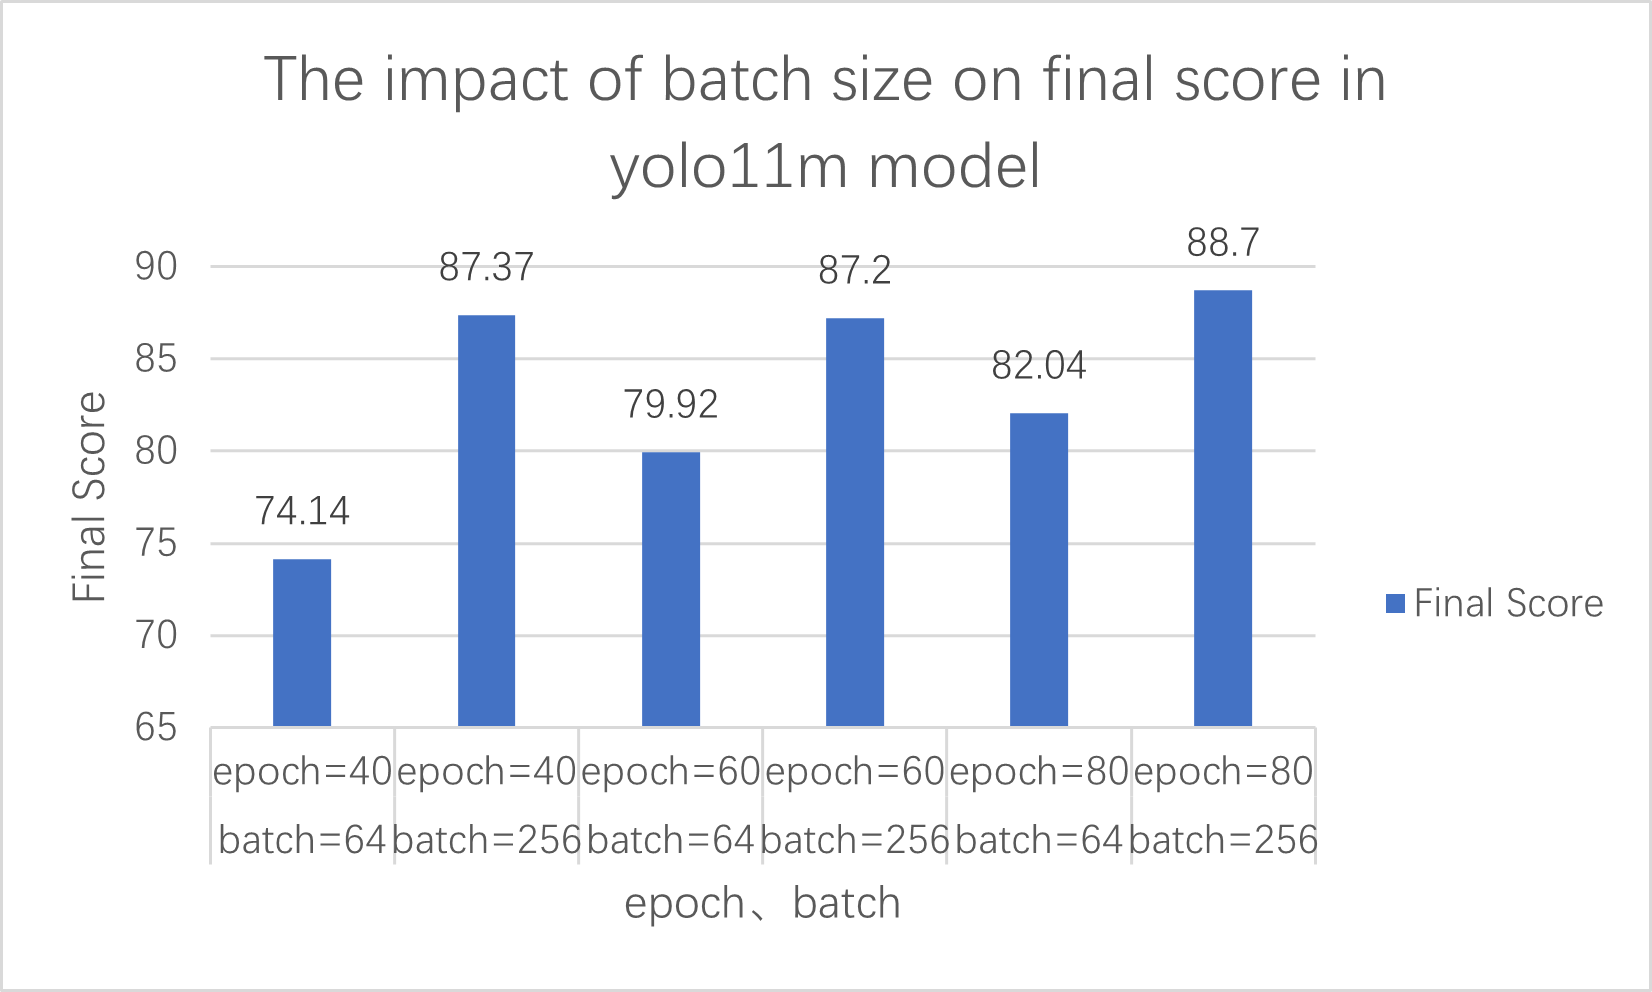
\includegraphics[width=0.8\linewidth]{./graphs/图片8.png}
  %\rule{0.9\linewidth}{0pt}
  %}

  \caption{Impact of Batch Size in YOLO11m Model}
  \label{fig:yolo-batchsize}
\end{figure}

From the chart, it is clear that increasing the batch size greatly helps the model's score, with a significant improvement. Increasing the batch size greatly enhances the model's ability under the same number of epochs.

With a batch size of 256, we increase the training epochs and obtain the line chart of prediction scores as epochs increase \cref{fig:yolo-epoch}.
\begin{figure}[t]
  \centering
  %\fbox{\rule{0pt}{2in}
  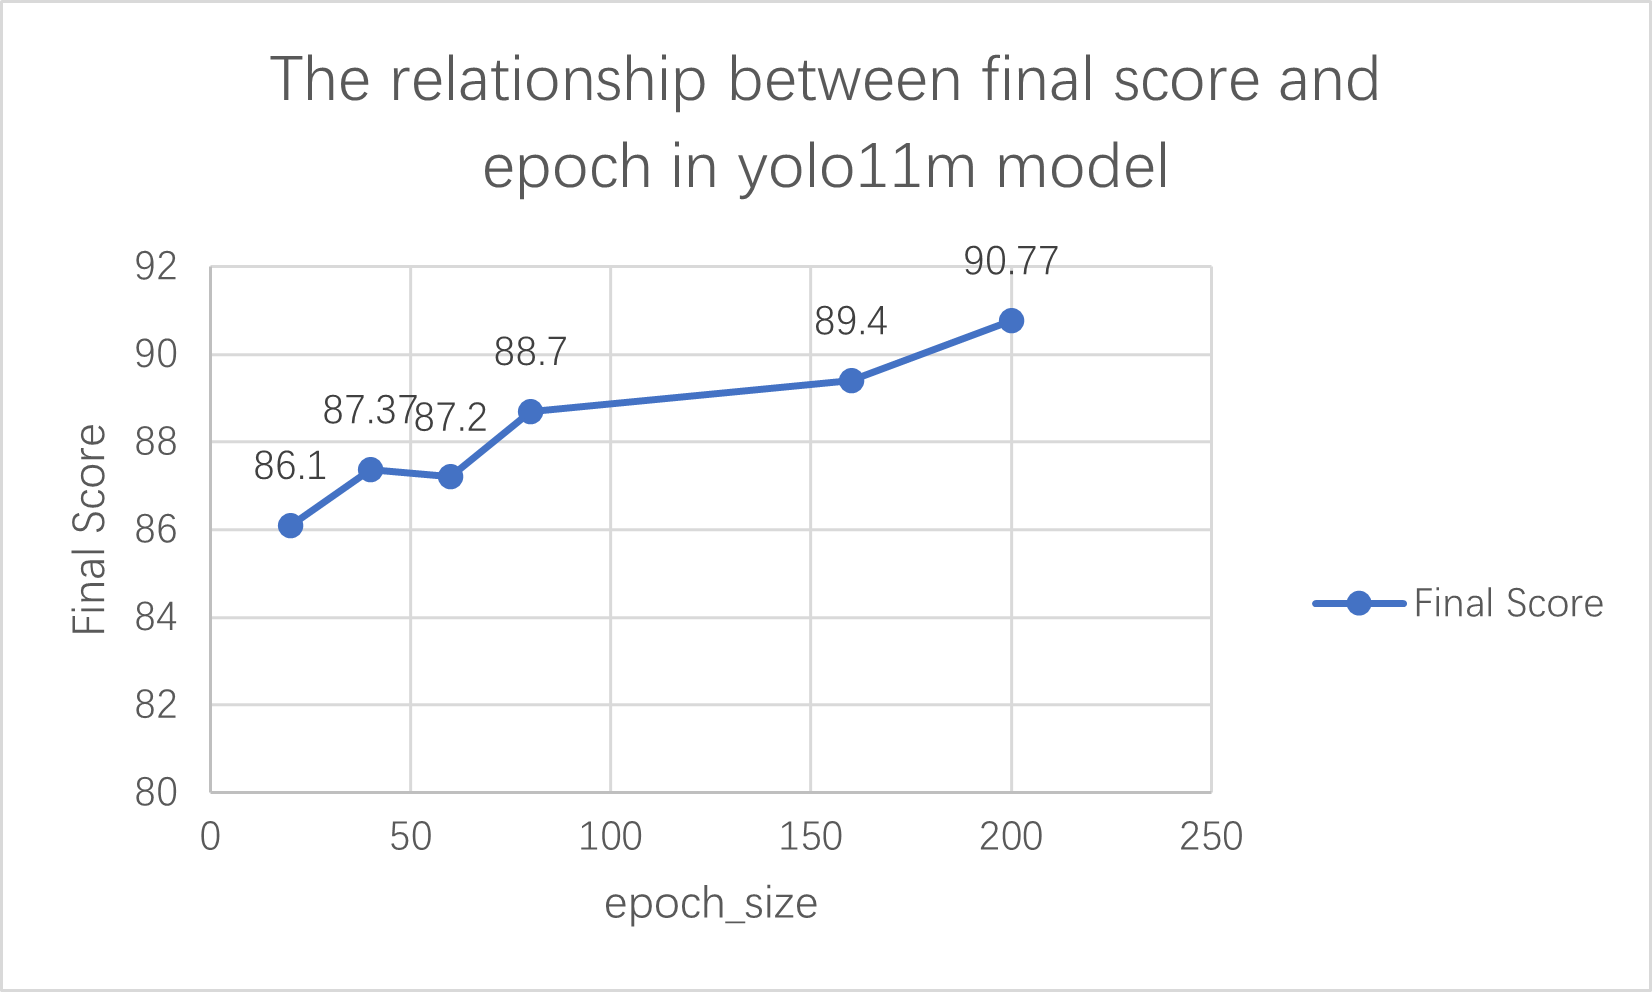
\includegraphics[width=0.8\linewidth]{./graphs/图片9.png}
  %\rule{0.9\linewidth}{0pt}
  %}

  \caption{Micro-F1 vs. Epochs for YOLO11m Model}
  \label{fig:yolo-epoch}
\end{figure}

From the chart, it can be seen that the YOLO11m model with batch = 256 is very powerful. While there are slight fluctuations during the increase in epochs, the overall trend is an upward one. At epoch = 200, the Micro-F1 score exceeds 90, which is a very high accuracy.

After adjusting the batch size and training epochs to make the model converge, we fine-tune the model by adjusting the confidence threshold ($conf$) and uniform image size ($image\_size$) to achieve a slight improvement in the score.

We set confidence thresholds to 0.3, 0.5, and 0.7, and compare the predicted results for epochs 50 and 200, as shown in the bar chart \cref{fig:yolo-conf}.

\begin{figure}[t]
  \centering
  %\fbox{\rule{0pt}{2in}
  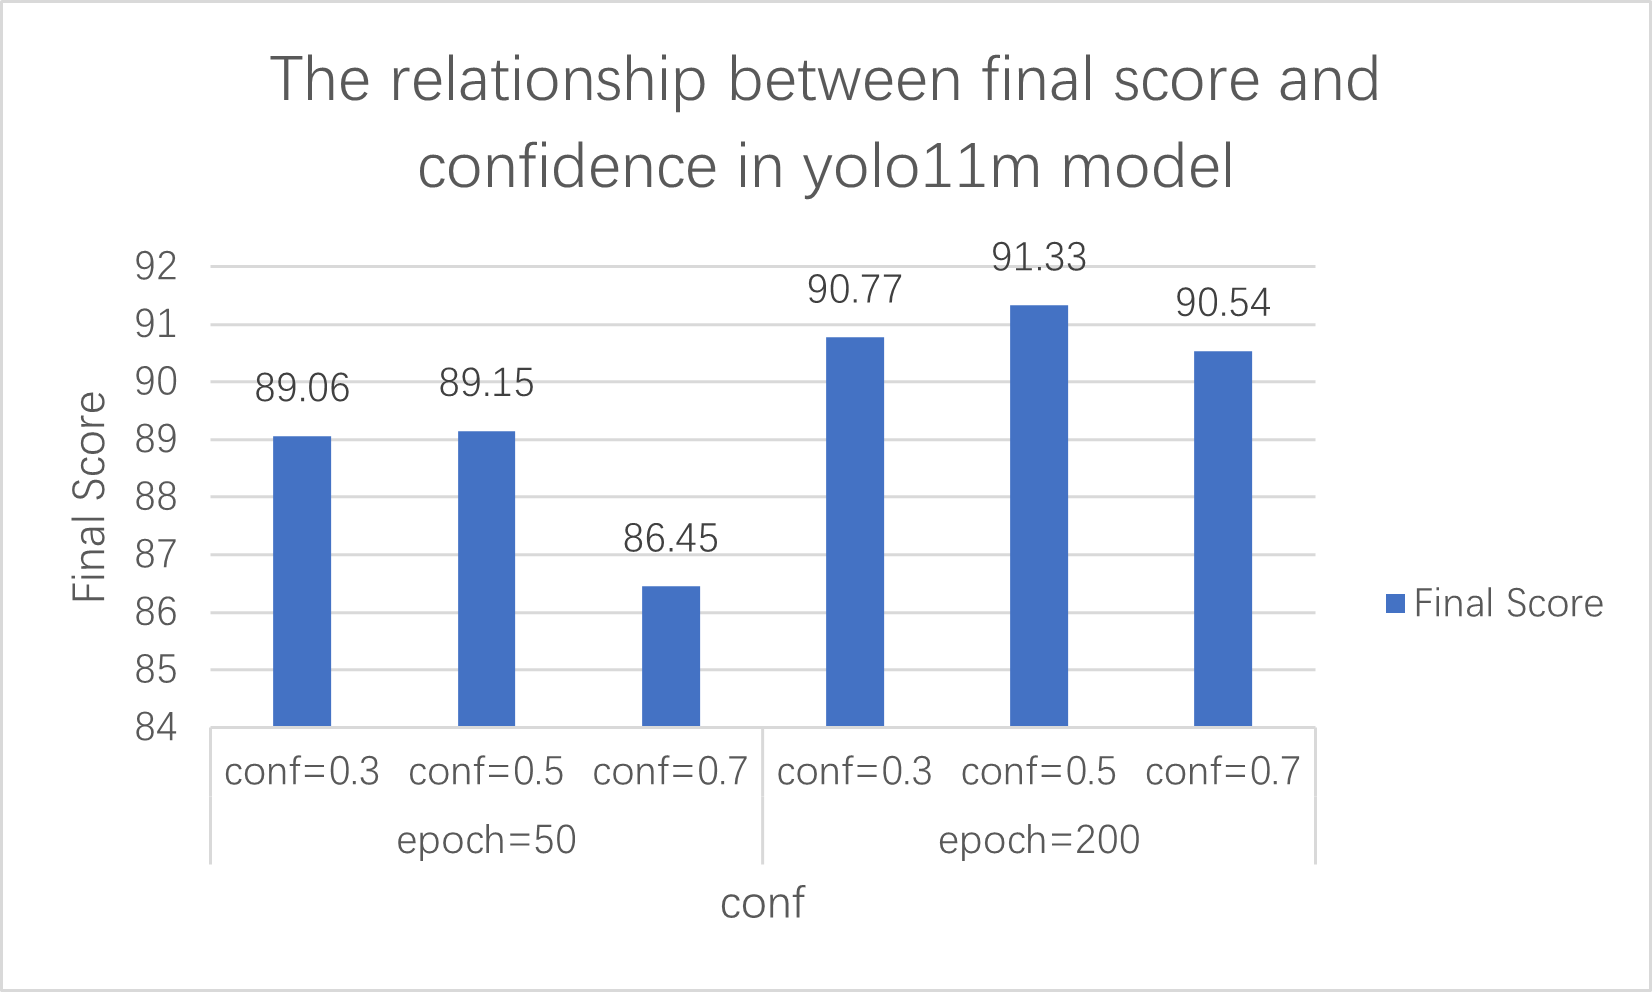
\includegraphics[width=0.8\linewidth]{./graphs/图片10.png}
  %\rule{0.9\linewidth}{0pt}
  %}

  \caption{Micro-F1 vs. Confidence Threshold in YOLO11m}
  \label{fig:yolo-conf}
\end{figure}

From the chart, it can be roughly seen that there is no definite pattern or conclusion between the confidence threshold and the model's score. Both too high and too low confidence thresholds lead to a decrease in model performance. The optimal confidence threshold varies after each training session. Therefore, confidence can only be used as a trial-and-error method to improve the model after finding the best one, and cannot directly determine the optimal confidence threshold for the model.

The results obtained from further testing, not shown in the figure, indicate that the model score reaches its optimal value of 93.68 when adjusting $conf = 0.2$.

Finally, we increase $image\_size$ to 800, which is the uniform size to which the images are scaled before training in the YOLO model. We compare the predicted results for epochs 150 and 200, as shown in the bar chart \cref{fig:yolo-size}.
\begin{figure}[t]
  \centering
  %\fbox{\rule{0pt}{2in}
  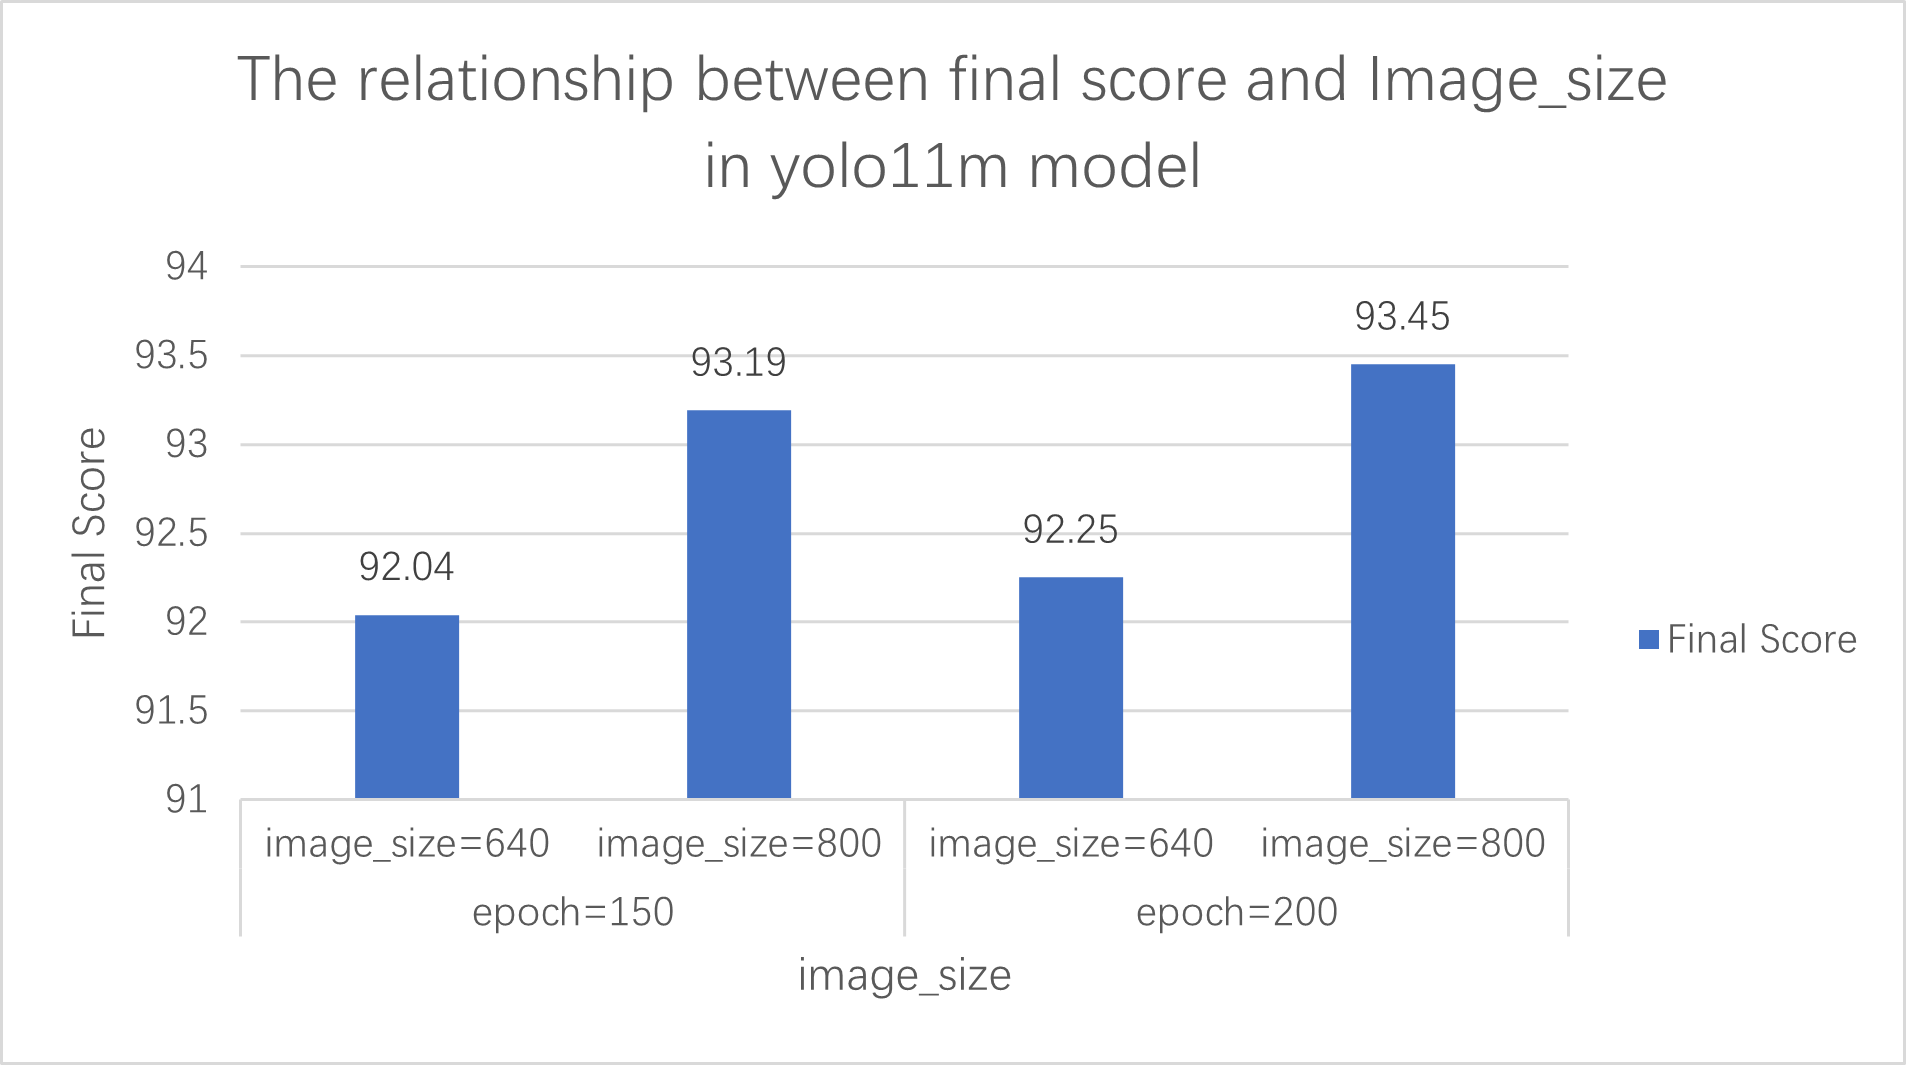
\includegraphics[width=0.8\linewidth]{./graphs/图片11.png}
  %\rule{0.9\linewidth}{0pt}
  %}

  \caption{Micro-F1 vs. Image Size in YOLO11m Model}
  \label{fig:yolo-size}
\end{figure}

Increasing the image size, though requiring more computing power, leads to better model performance because more information is preserved in the images.

\subsubsection{Innovation 3: Multi-scale Data Augmentation}

Due to data augmentation operations such as image flipping, the data volume can be expanded to make the network-trained model more accurate\cite{sym11101223}, which proved feasible for optimizing the scores. Therefore, we also tried multi-scale data augmentation.

To enhance the model's robustness to tampering at different scales, we introduce multi-scale image resizing during the training of YOLO11m. The data augmentation parameter configuration is shown in \cref{fig:yolo-data-code}.
\begin{figure}[t]
  \centering
  %\fbox{\rule{0pt}{2in}
  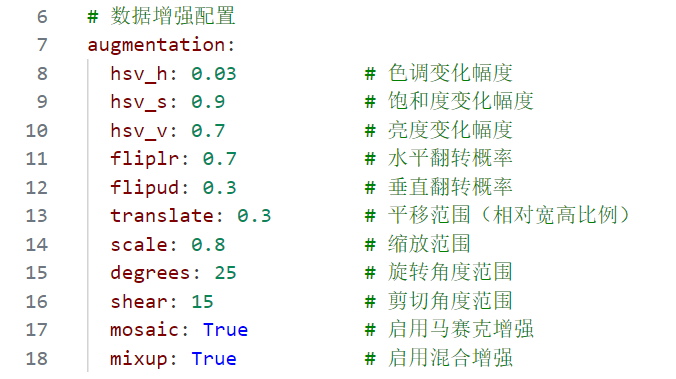
\includegraphics[width=0.8\linewidth]{./graphs/图片6.png}
  %\rule{0.9\linewidth}{0pt}
  %}

  \caption{Data Augmentation Parameter Configuration}
  \label{fig:yolo-data-code}
\end{figure}

We compare the prediction scores for epochs 150 and 200 with and without data augmentation, as shown in the bar chart \cref{fig:yolo-data}.
\begin{figure}[t]
  \centering
  %\fbox{\rule{0pt}{2in}
  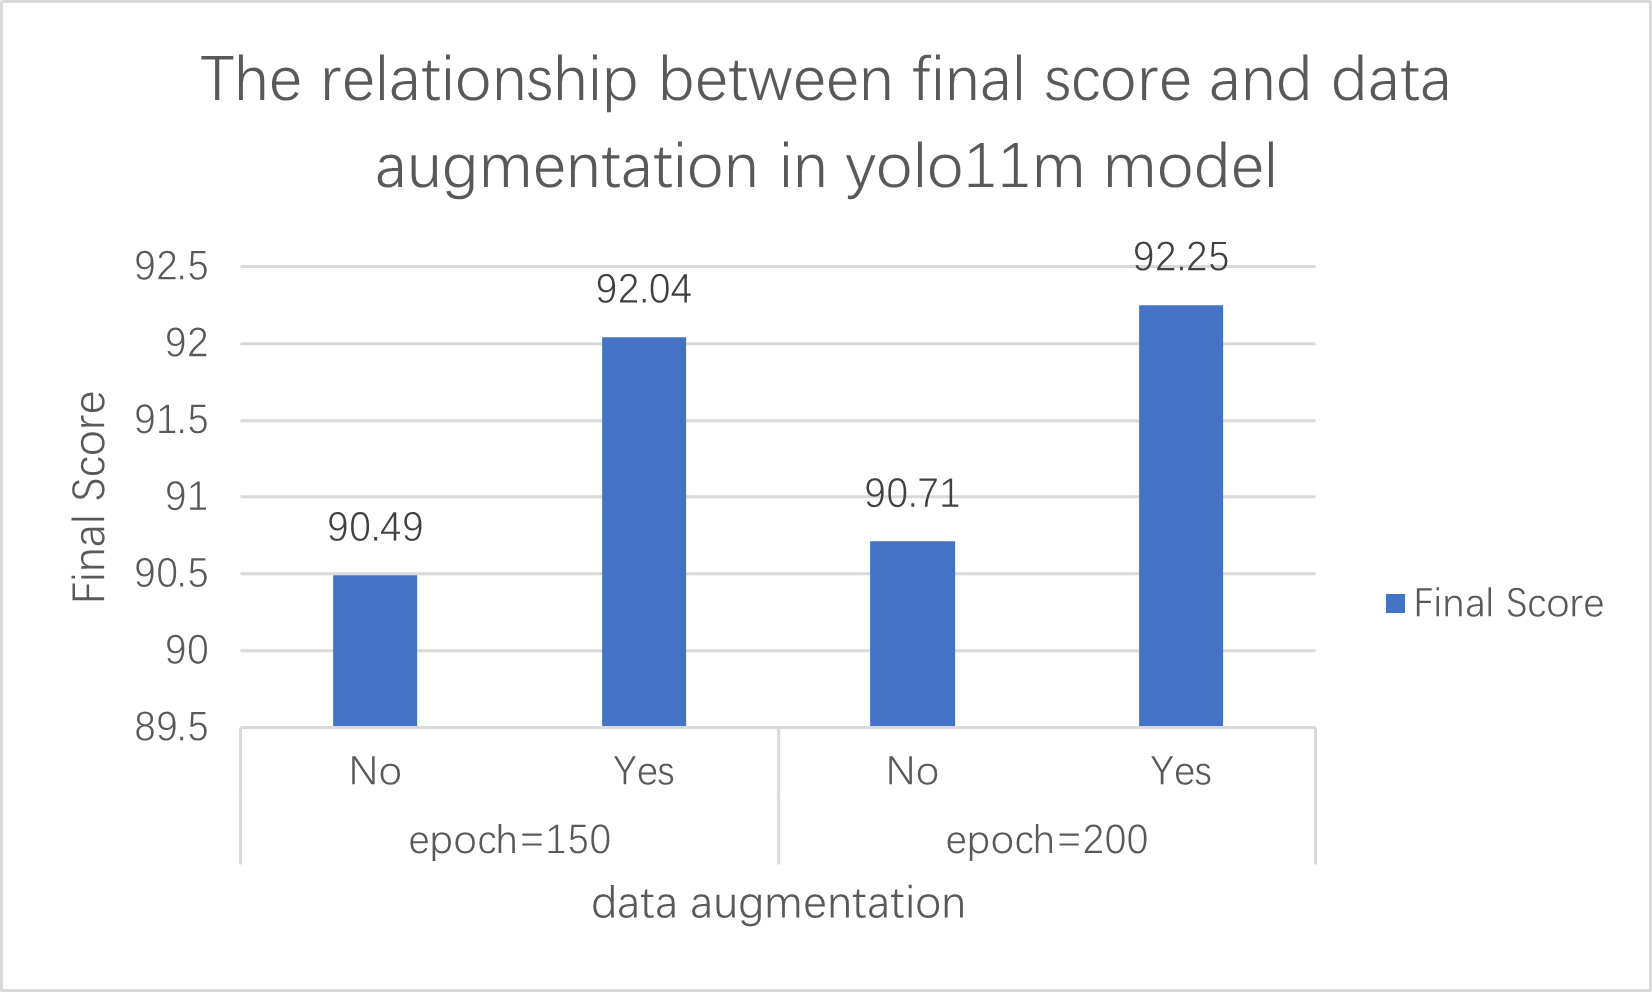
\includegraphics[width=0.8\linewidth]{./graphs/图片7.png}
  %\rule{0.9\linewidth}{0pt}
  %}

  \caption{Micro-F1 vs. Data Augmentation in YOLO11m Model}
  \label{fig:yolo-data}
\end{figure}

Before data augmentation, no matter what tuning method was applied, the highest score the model could achieve was 90.71. However, with data augmentation and the same training parameters, the model score reached 92.25, indicating that data augmentation has a significant effect on the YOLO model.

\subsection{Ablation Experiment Results}

Based on the comparisons in \cref{subsec:create} between Faster R-CNN models with and without region threshold filtering and parameter adjustments, and YOLO models with and without multi-scale data augmentation and parameter adjustments, we present the results in tables \cref{tab:xiaorong} and \cref{tab:xiaorong2} using Micro-F1 as the metric.

\begin{table}
  \centering
  \begin{tabular}{c|c|c|c}
    \toprule
    Model                         & Filter & Adjustment & Micro-F1 \\
    \midrule
    \multirow{3}{*}{Faster R-CNN} & No     & No         & 56.06    \\
                                  & No     & Yes        & 67.89    \\
                                  & Yes    & Yes        & 70.84    \\
    \bottomrule
  \end{tabular}
  \caption{Ablation Experiment Results Table for Faster R-CNN}
  \label{tab:xiaorong}
  \vspace{\baselineskip}
  \begin{tabular}{c|c|c|c}
    \toprule
    Model                 & Augmentation & Adjustment & Micro-F1 \\
    \midrule
    \multirow{3}{*}{YOLO} & No           & No         & 76.84    \\
                          & No           & Yes        & 90.71    \\
                          & Yes          & Yes        & 93.68   \\
    \bottomrule
  \end{tabular}
  \caption{Ablation Experiment Results Table for YOLO}
  \label{tab:xiaorong2}
\end{table}

Region threshold filtering significantly improved Faster R-CNN's performance on smaller tampered regions.

Multi-scale data augmentation improved YOLO11m's generalization ability across different tampering patterns.

Adjusting training parameters and configuration files also resulted in an increase in score over the model's baseline.
